\section{Informe Web API} 
\begin{flushleft}


\begin{itemize}
\textbf{Parte1: Creación del servicio REST Web API }\\
\textbf{ }\\
  \item Paso 1. De la categoría Web, selecciona el proyecto de tipo ASP.NET Web Application (.NET Framework) y coloca el nombre AlumnosWebApp.

\begin{center}
	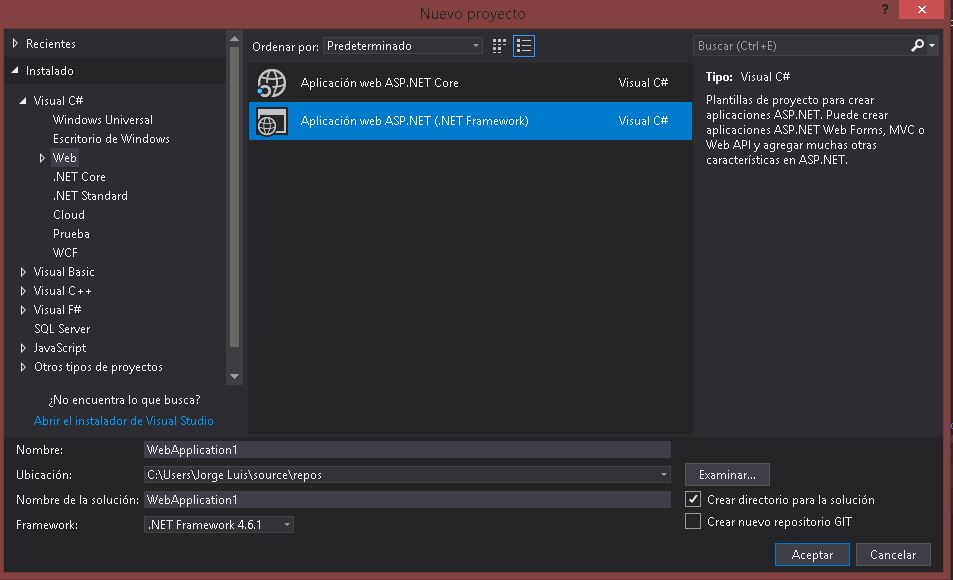
\includegraphics[width=16cm]{./Imagenes/paso1} 
	\end{center}
\textbf{ }\\
\item Paso 2. Selecciona el template Web API y da clic en OK.
\begin{center}
	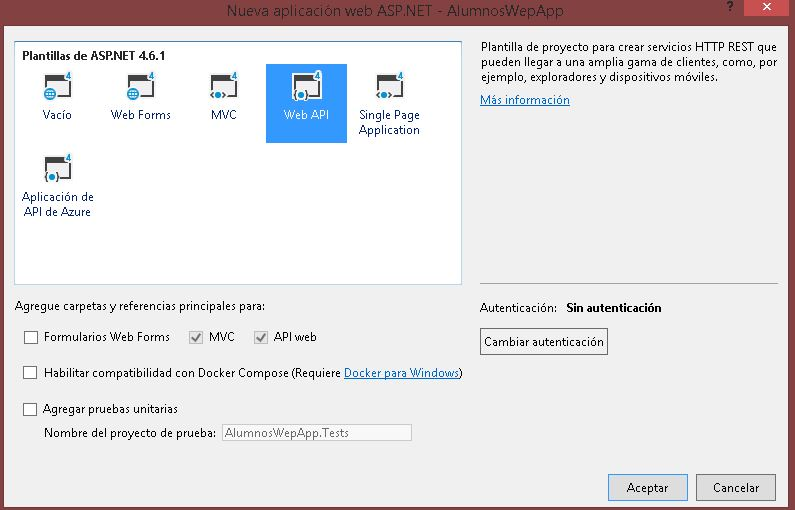
\includegraphics[width=12cm]{./Imagenes/paso2} 
	\end{center}

\textbf{ }\\
\item Paso 3. Agregar las clases en la carpeta Models. Estas clases representan las tablas que vamos a agregar a nuestra base de datos. Las propiedades representan los campos de la tabla. El código es el siguiente:
\begin{center}
	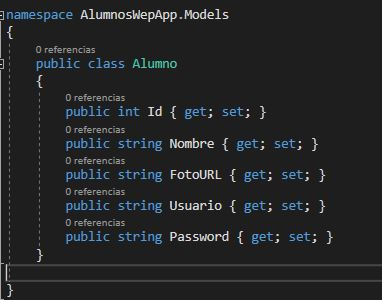
\includegraphics[width=12cm]{./Imagenes/paso3} 
	\end{center}
\textbf{ }\\
\item Paso 4. En la carpeta Modelos agrega otra clase llamada Tarea. Al igual que en el caso anterior, ésta es
otra tabla que incluiremos en nuestra base de datos, con el código siguiente: 
\begin{center}
	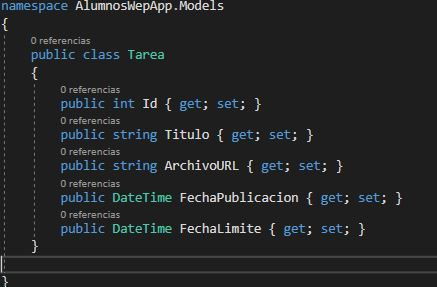
\includegraphics[width=12cm]{./Imagenes/paso4} 
	\end{center}

\textbf{ }\\
\textbf{ }\\
\item Paso 5. Como última tabla, en nuestra carpeta Modelos agrega una clase llamada TareaAlumno, la cual
representa una relación de N a N entre las tablas anteriores (Alumno y Tarea). Esto lo representaremos
con los atributos ForeignKey y Key en las propiedades de ID, así como un elemento virtual para
navegación estilo EntityFramework.

\begin{center}
	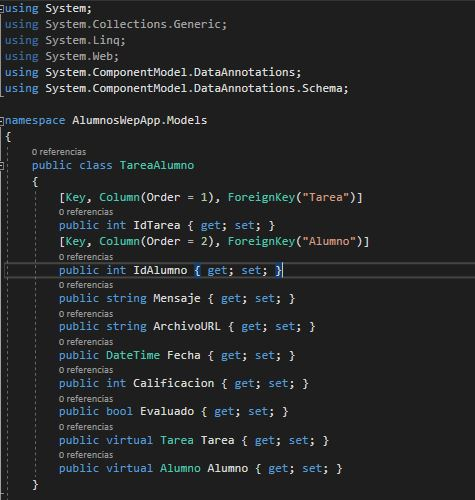
\includegraphics[width=12cm]{./Imagenes/paso5} 
	\end{center}

\textbf{ }\\
Como puedes intuir, las clases creadas son modelos de tablas que serán generadas en una base de datos. 
\textbf{ }\\
\textbf{ }\\
\textbf{ }\\
\textbf{ }\\
\textbf{ }\\
\item Paso 6. Después de crear tus modelos, compila la solución.
\begin{center}
	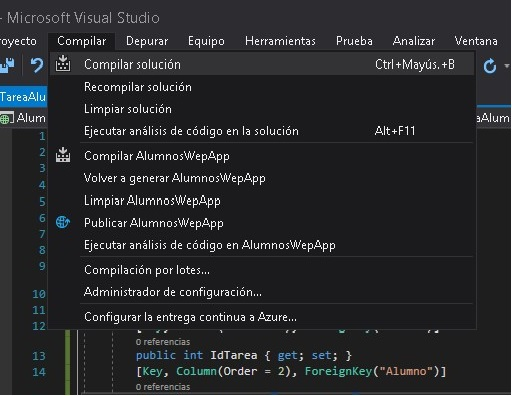
\includegraphics[width=12cm]{./Imagenes/paso6} 
	\end{center}

\item  Paso 7. Ahora da clic derecho en la carpeta Controllers y agrega un nuevo Controlador

\begin{center}
	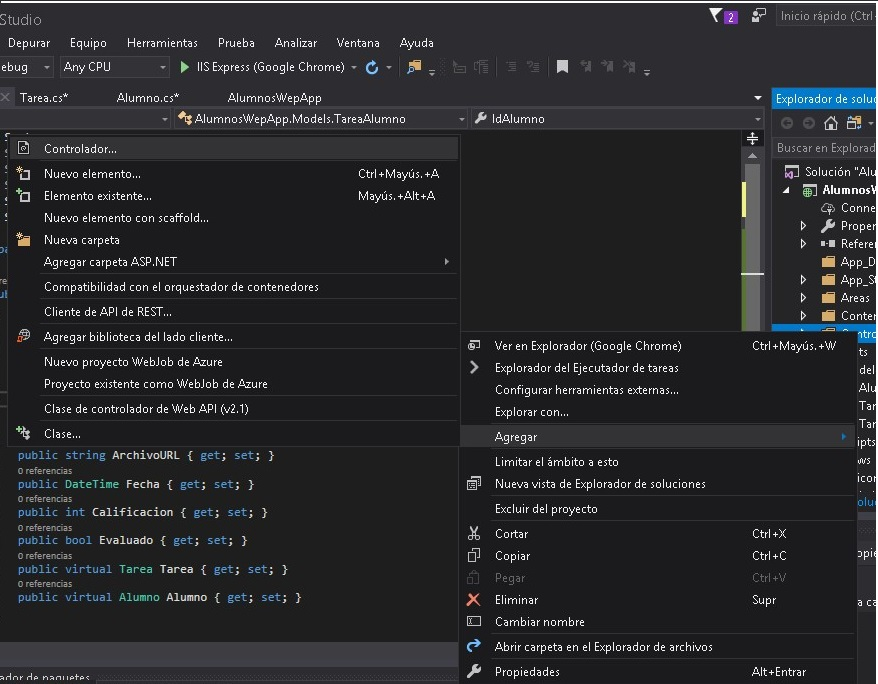
\includegraphics[width=12cm]{./Imagenes/paso7} 
	\end{center}
\textbf{ }\\
\textbf{ }\\
\textbf{ }\\
\textbf{ }\\
\item Paso 8. Selecciona Web API 2 Controller with actions, using EntityFramework en la categoría de Scaffolds
\begin{center}
	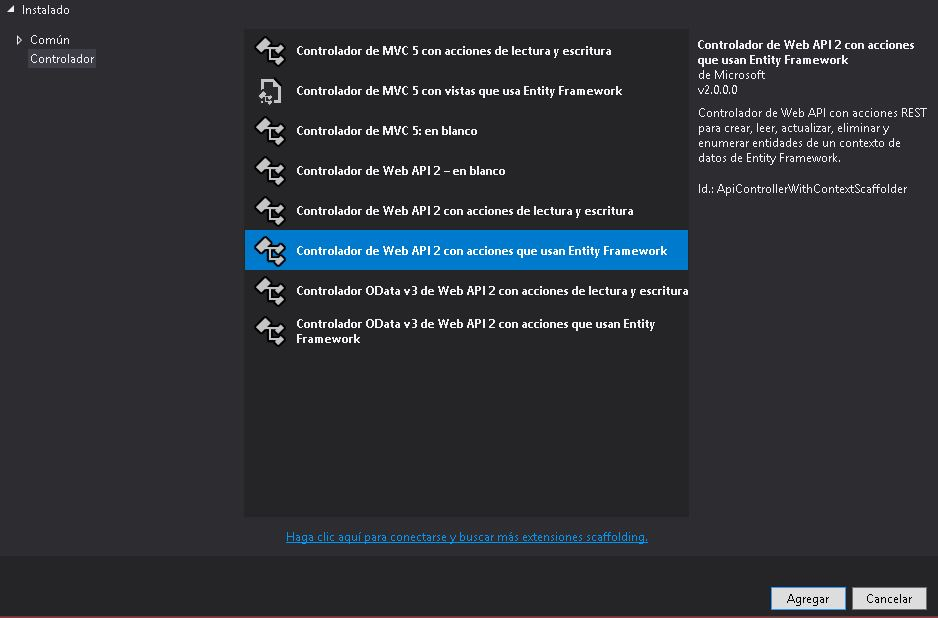
\includegraphics[width=12cm]{./Imagenes/paso8} 
	\end{center}

\item Paso 9. En clase de Modelo selecciona Alumno y da clic en el botón + para agregar una clase de contexto
(conexión).
\begin{center}
	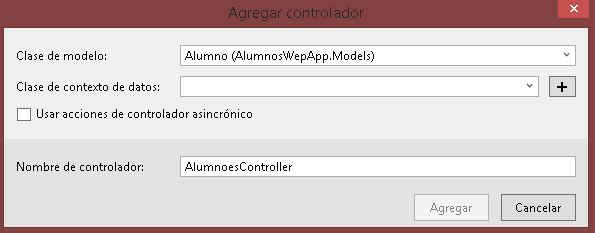
\includegraphics[width=12cm]{./Imagenes/paso9} 
	\end{center}

\item Paso 10. Da clic en Agregar (el nombre de la clase de contexto no es relevante, se recomienda dejarlo
como aparece): 
\begin{center}
	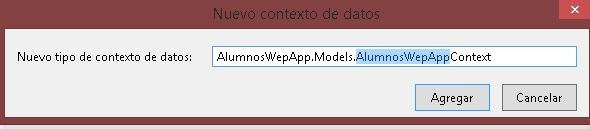
\includegraphics[width=12cm]{./Imagenes/paso10} 
	\end{center}

\textbf{ }\\
\textbf{ }\\
\textbf{ }\\
\textbf{ }\\
\item Paso 11. De regreso en la pantalla de Agregar Cotrolador, modifica el nombre del controlador a
AlumnosController y da clic en Agregar.
\begin{center}
	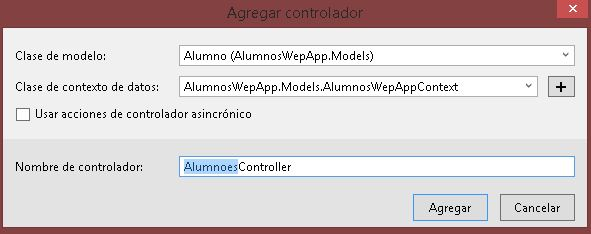
\includegraphics[width=12cm]{./Imagenes/paso11} 
	\end{center}

\item Paso 12. Modifica o agrega los siguientes métodos dentro del controlador:
\begin{center}
	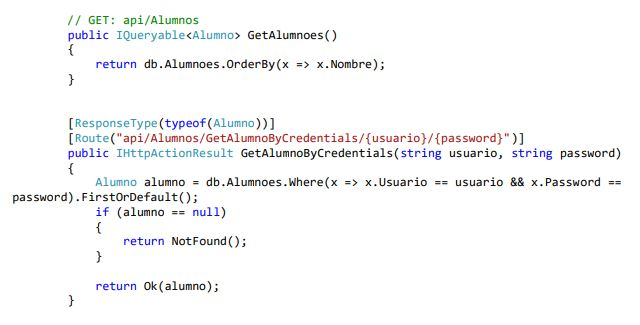
\includegraphics[width=12cm]{./Imagenes/paso12} 
	\end{center}

\item Paso 13. Agrega otro controlador con la siguiente información: 
\begin{center}
	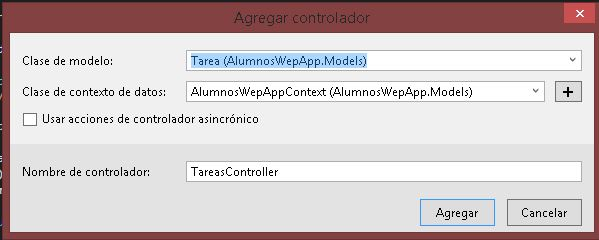
\includegraphics[width=12cm]{./Imagenes/paso13} 
	\end{center}

\item Paso 14. Modifica el método GetTareas: 

\begin{center}
	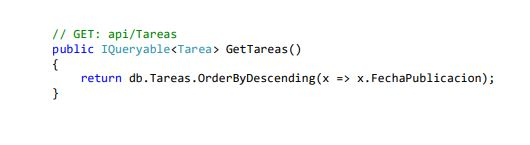
\includegraphics[width=12cm]{./Imagenes/paso14} 
	\end{center}

Paso 15. Agrega otro controlador con la siguiente información: 
\begin{center}
	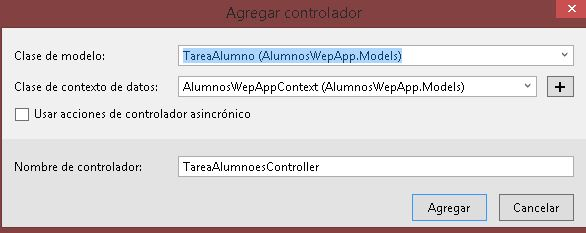
\includegraphics[width=12cm]{./Imagenes/paso15} 
	\end{center}

Paso 16. El código completo del controlador se muestra a continuación: 

\begin{center}
	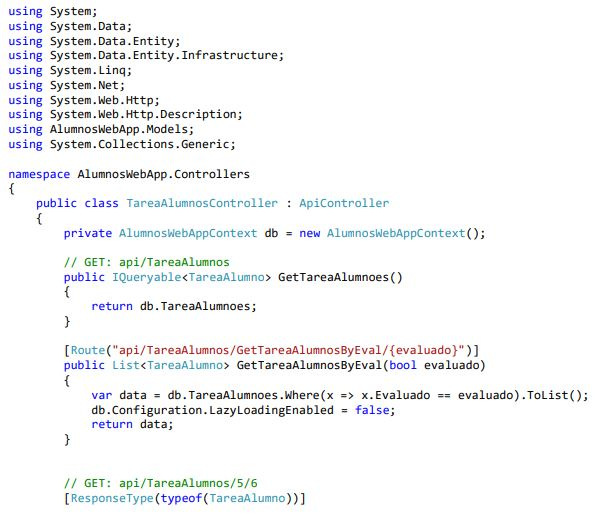
\includegraphics[width=12cm]{./Imagenes/paso16} 
	\end{center}

\textbf{ }\\

\begin{center}
	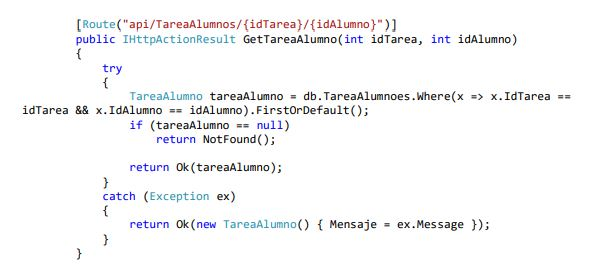
\includegraphics[width=12cm]{./Imagenes/paso16-1} 
	\end{center}

\textbf{ }\\

\begin{center}
	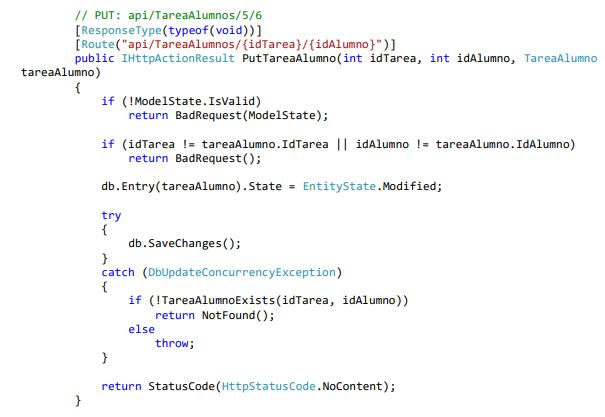
\includegraphics[width=12cm]{./Imagenes/paso16-2} 
	\end{center}

\textbf{ }\\

\begin{center}
	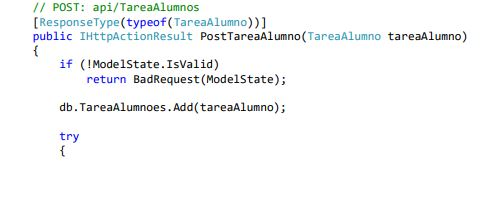
\includegraphics[width=12cm]{./Imagenes/paso16-3} 
	\end{center}

\textbf{ }\\

\begin{center}
	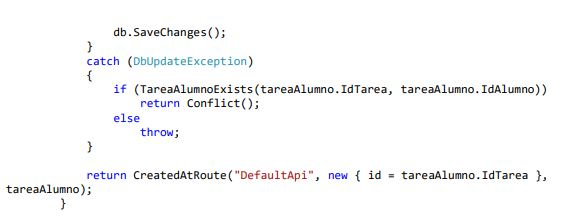
\includegraphics[width=12cm]{./Imagenes/paso16-4} 
	\end{center}
\textbf{ }\\

\begin{center}
	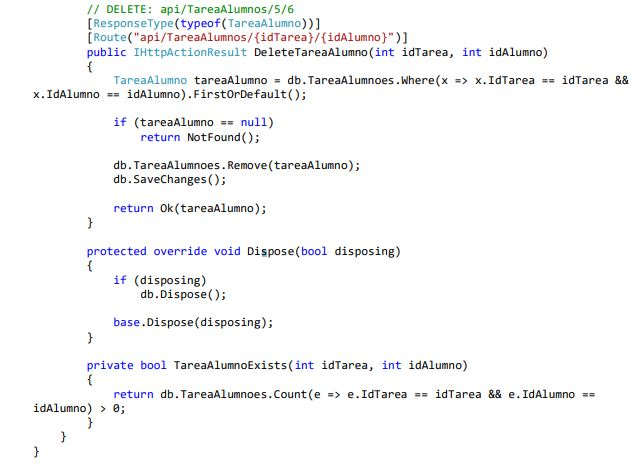
\includegraphics[width=12cm]{./Imagenes/paso16-5} 
	\end{center}


\item Paso 17. Compila y ejecuta la aplicación: 

\begin{center}
	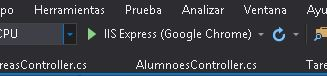
\includegraphics[width=12cm]{./Imagenes/paso17} 
	\end{center}

\item Paso 18. Da clic en el enlace API a fin de observar la descripción de los controladores de nuestra aplicación: 
\begin{center}
	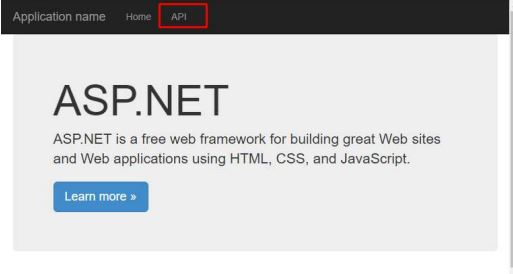
\includegraphics[width=12cm]{./Imagenes/paso18} 
	\end{center}

\item Paso 19. Localiza el controlador Alumnos y sus métodos. Da clic en POST Alumnos para agregar un
registro:
\begin{center}
	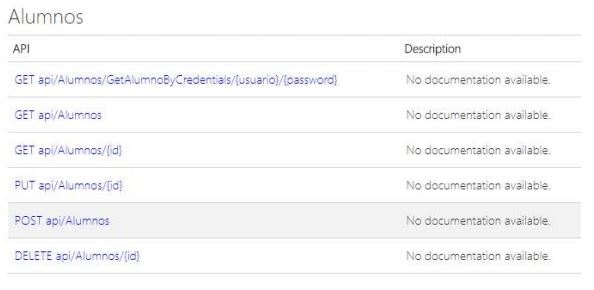
\includegraphics[width=12cm]{./Imagenes/paso19} 
	\end{center}

\item Paso 20. Observa el formato de la cadena que debe ser enviada y cópiala:
\begin{center}
	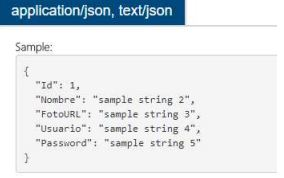
\includegraphics[width=12cm]{./Imagenes/paso20} 
	\end{center}

\item Paso 21. Ahora abre la aplicación Postman y sigue los pasos para hacer una petición POST al servicio, lo
cual nos permitirá agregar un nuevo alumno en nuestra base de datos: 
\begin{center}
	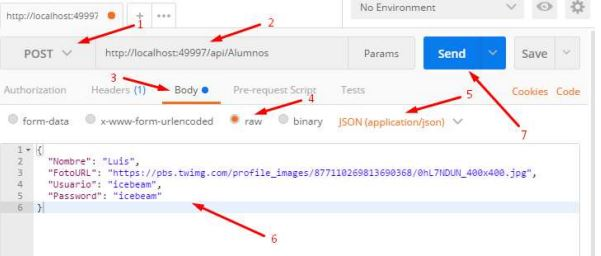
\includegraphics[width=12cm]{./Imagenes/paso21} 
	\end{center}

\item Paso 22. Si hacemos una petición GET al api de Alumnos, podemos comprobar que el registro ha sido
agregado con éxito:
\begin{center}
	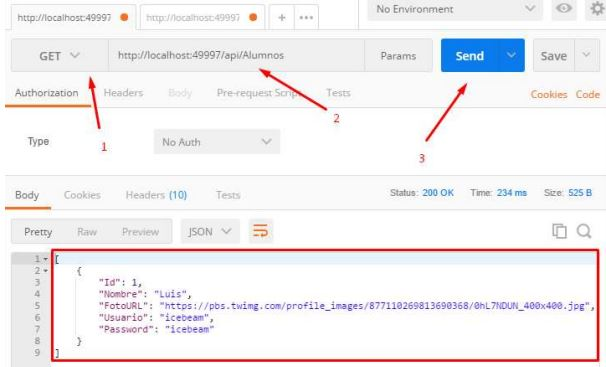
\includegraphics[width=12cm]{./Imagenes/paso22} 
	\end{center}


\item Paso 23. Ahora agrega una nueva Tarea. Primero damos clic en el POST del api de Tareas
\begin{center}
	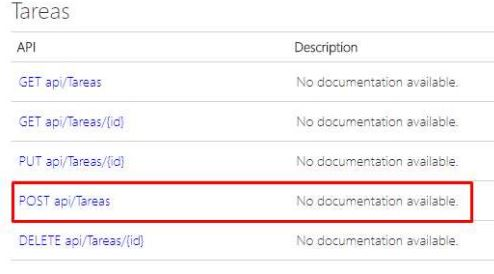
\includegraphics[width=12cm]{./Imagenes/paso23} 
	\end{center}


\item Paso 24. Observamos el formato de la cadena JSON a introducir: 
\begin{center}
	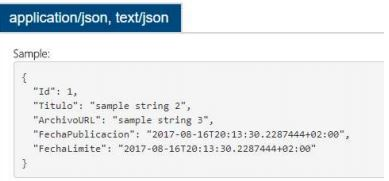
\includegraphics[width=12cm]{./Imagenes/paso24} 
	\end{center}

\item Paso 25. Observamos el formato de la cadena JSON a introducir: 
\begin{center}
	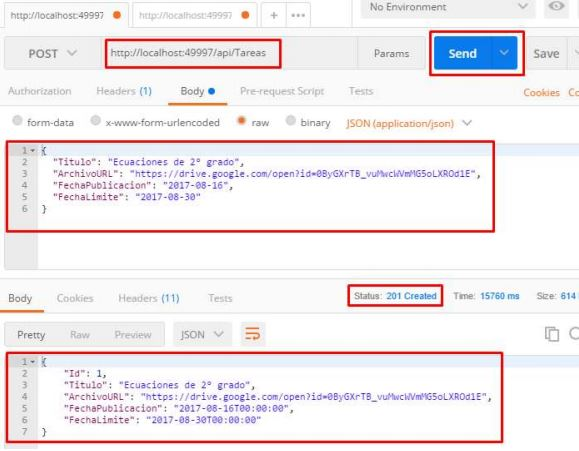
\includegraphics[width=12cm]{./Imagenes/paso25} 
	\end{center}

\item Paso 26.  Finalmente, comprobamos que también funcione el api de TareaAlumnos. Para ello, damos clic
en POST dicho api:
\begin{center}
	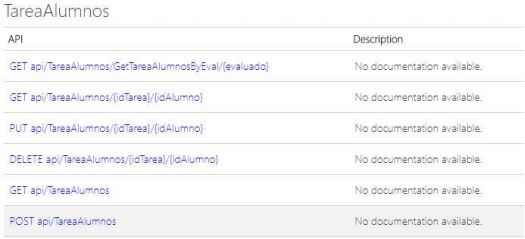
\includegraphics[width=12cm]{./Imagenes/paso26} 
	\end{center}

\item Paso 27.  Verificamos la cadena JSON, centrándonos únicamente en las propiedades que no son de
navegación:
\begin{center}
	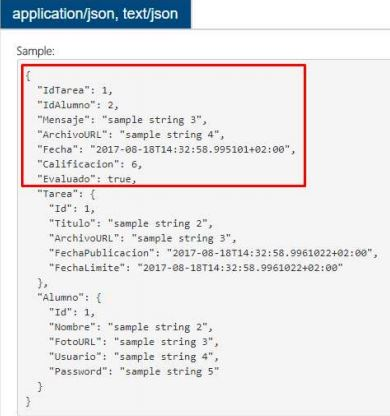
\includegraphics[width=12cm]{./Imagenes/paso27} 
	\end{center}



\item Paso 28.  Hacemos la petición POST al api de TareaAlumnos en Postman:
\begin{center}
	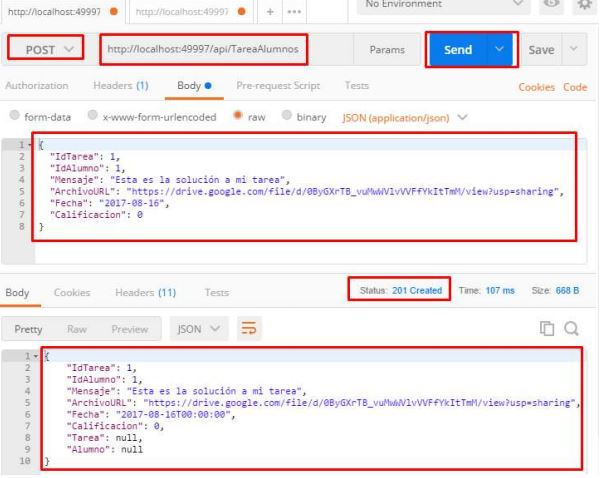
\includegraphics[width=12cm]{./Imagenes/paso28} 
	\end{center}

\item Paso 29.   Comprobamos que ha sido agregado un nuevo registro en la tabla:
\begin{center}
	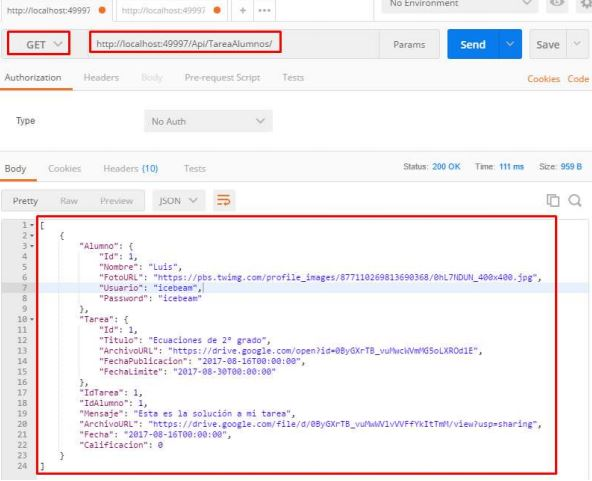
\includegraphics[width=12cm]{./Imagenes/paso29} 
	\end{center}

\end{itemize} 


\end{flushleft}